\documentclass[11pt]{article}

\usepackage{graphicx}
\usepackage{polski}
\usepackage[utf8]{inputenc}

\title{LearnIt - dokumentacja \\ \large Programowanie obiektowe 2017}
\author{Maciej Draguła}
\date{czerwiec 2017}

\begin{document}

\makeatletter
    \begin{titlepage}
        \begin{center}
            
\includegraphics[width=0.7\linewidth]{UWr.png}\\[10ex]
            {\huge \bfseries  \@title }\\[6ex] 
            {\LARGE  \@author}\\[50ex] 
            {\large \@date}
        \end{center}
    \end{titlepage}
\makeatother
\thispagestyle{empty}
\newpage


\section{Alfabetyczny spis klas}
\begin{itemize}
	\item Base
	\item Exercise1
	\item Exercise2
	\item Exercise3
	\item Exercise4
	\item Frame
	\item Intro
	\item Login
	\item MainProgram
	\item NewUserWindow
	\item StartWindow
	\item UserMenu
	\item WhatToLearn
\end{itemize}

\section{Opis projektu oraz poszczególnych klas}
\subsection{Ogólny opis projektu}
LearnIt jest niewielką aplikacją komputerową służącą do nauki słówek i haseł za pomocą tzw. fiszek. Program został stworzony jako projekt końcowy na przedmiocie \textit{Programowanie Obiektowe} na Uniwersytecie Wrocławskim w semestrze letnim roku akademickiego 2016/2017 przez Agnieszkę Dudek, Julię Majkowską oraz Macieja Dragułę. Jest on napisany w języku Java z wykorzystaniem biblioteki graficznej Swing. \\\\
Po uruchomieniu programu widoczne jest okno logowania. Użytkownik powinien założyć konto klikając przycisk \textit{New user}. Po wybraniu nazwy użytkownika i hasła należy zatwierdzić stworzenie użytkownika przyciskiem \textit{Create new account}. Po zapoznaniu się z ogólnymi wskazówkami należy wybrać, czy użytkownik chce załadować istniejącą bazę z pliku, czy też stworzyć własną. Podczas tworzenia własnej bazy mamy możliwość, oprócz obowiązkowych pól takich jak: \textit{Category}, \textit{Phrase}, \textit{Meaning}, dodać własne. Po zapisaniu nowostworzonej bazy należy zapsiać ją do pliku i załadować. Następnie otwiera się nowe menu, w którym możemy wybrać, czy chcemy dodać nowe fiszki do załadowanej bazy (przycisk \textit{Add}), uczyć się nowych albo powtarzać wcześniej przyswojone. \\\\
W trybie \textit{Learn} użytkownik winien wybrać kategorię oraz liczbę fiszek, których chce się uczyć (dostępna jest opcja \textit{wszytskie}). Tryb \textit{Learn} jest podzielony na cztery etapy. W pierwszym program wyświetla hasła oraz ich znaczenia, należy wtedy próbować zapamiętać frazy. Użytkownik sam decydyje, kiedy chce uczyć się kolejnego słówka klikając przycisk \textit{Continue}. Następnie rozpoczyna się pierwsze ćwiczenie, w którym zostaje wyświetlone pytanie, a po kliknięciu \textit{Show answer} odpowiedź. Użytkownik sam decyduje, czy zapamiętał hasło czy nie klikając jeden z przycisków: \textit{Fail} lub \textit{OK}. Potem następuje druga faza nauki, w której wyświetlona jest część odpowiedzi i należy uzupełnić ją brakującymi literkami. W przypadku błędnego wprowadzenia tekstu należy kliknąć \textit{Reset answer}. Program weryfikuje poprawność odpowiedzi i w przypadku błędu wyświetli poprawne rozwiązanie. W czwartej fazie nauki użytkownik otrzymuje ćwiczenie, w którym, bez żadnych podpowiedzi, powinien wprowadzić odpowiedź na zadane pytanie lub przetłumaczyć frazę. Podobnie jak w fazie trzeciej w przypadku błędnej odpowiedzi program wyświetli użytkownikowi prawidłową odpowiedź. Jeżeli na któreś z ćwiczeń została udzielona niepoprawna odpowiedź, program doda fiszkę na koniec kolejki pytań i będzie to robił tak długo, aż użytkownik nie udzieli bezbłędnych odpowiedzi.\\\\
Tryb \textit{Repeat} służy do powtarzania haseł poznanych w trybie \textit{Learn}. Program, w zależności od poprawności odpowiedzi użytkownika, sam decyduje w jakim odstępie czasowym dane słówko należy powtórzyć. Odstęp jest wydłużany przy kolejnych poprawnych odpowiedziach oraz skracaniu przy błędnych.

\subsection{Opis mojej części pracy}
Jak każdy członek zespołu brałem udział w projektowaniu całego programu, natomiast moim głównym zadaniem była implementacja interfejsu graficznego z wykorzystaniem biblioteki Swing. Prawie wszytskie stworzone przeze mnie klasy są rozszerzeniem klasy \textit{JPanel} lub \textit{JFrame}. Obiekty stwarzane przeze mnie w programie są w większości kontenerami, które wyświetlają menu albo fiszki podawane przez algorytm Agnieszki Dudek. Niektóre klasy bezpośrendnio implementują interfejsy \textit{ActionListener} oraz \textit{ChangeListener}, do innych natomiast jest przekazywana referencja do obiektu klasy \textit{Frame}, którego głównym zadaniem jest odbieraniem sygnałów od kolejnych przysisków. \\
Każda stworzona klasa rozszerzająca \textit{JPanel} korzysta z managera layoutów o nazwie \textit{GridBagLayout}. Za pomocą obiektu klasy \textit{GridBagConstraints} defniowałem położenie przycisków, etykiet oraz pól do wprowadzania tekstu, jak również rozmiar wcięć i dopasowanie pól do szerowości ramki.
Implemetacja interfejsu graficznego we wszytskich klasach sprowadza się do implementacji konstruktów oraz ewentualnie metody \textit{ActionPerformed} wymaganej przez interfejsy \textit{ActionListener} oraz \textit{ChangeListener}.

\subsection{Klasa: Base}
\subsubsection*{extends Jpanel}

Zadaniem klasy Base jest wyświetlenie dwóch przycisków, które pozwalają stworzyć nową bazę fiszek albo załadować z pliku. Informacja o sygnale pochodzącym od przycisków \textit{Create new base} oraz \textit{Load from file} jest przekazywana do obiektu klasy \textit{Frame}.

\subsection{Klasa: Exercise1}
\subsubsection*{extends Jpanel}

Klasa \textit{Exercise1} to interfejs ćwiczenia, w którym użytkownić musi samodzielnie wprowadzić odpowiedź z klawiatury. Argumentami konstruktora są referencje do aktualnie używanej ramki oraz do pytania. Panel składa się a dwóch podpanelów (panel pytania i panel odpowiedzi) oraz przycisku \textit{Continue}, z którego sygnał jest przekazywany do ramki. W panelu pytania umieszczona jest etykieta z pytaniem na białym tle, natomiast w panelu odpowiedzi znajduje się pole tekstowe do wprowadzania odpowiedzi.

\subsection{Klasa: Exercise2}
\subsubsection*{extends JPanel implements ActionListener}

Klasa \textit{Exercise2} to interfejs ćwiczenia, którym użytkownik odpowiada samodzielnie na zadane pytanie bądź tłumaczy frazę, a następnie wybiera, czy udzielił prawidłowej odpowiedzi. W konstruktorze tworzone są (podobnie jak w ćwiczeniu nr 1) panel pytania i odpowiedzi. W panelu z pytaniem umieszczona jest etykieta z pytaniem na białym tle. Panel pytania początkowo zawiera pustą etykietę z odpowiedzią. Poniżej panelów znajdują się przyciski \textit{Show answer}, \textit{Fail}, \textit{OK}, przy czym dwa ostatnie są początkowo ukryte.\\
Klasa implementuje interfejs \textit{ActionListener}, zatem jest również zaimplementowana metoda \textit{actionPerformed}. Przycisk \textit{Show answer} jest połączony z lokalnym Action Listenerem i po kilknięciu tego przycisku jest on ukrywany, natomiast pojawiają się przyciski \textit{Fail} oraz \textit{OK} połączone z ramką typu \textit{Frame}. Wtedy wyświetlana jest również odpowiedź.

\subsection{Klasa: Exercise3}
\subsubsection*{extends JPanel implements ActionListener}
Klasa \textit{Exercise3} to interfejs graficzny ćwiczenia, w którym użytkownik wprowadza tylko konkretne litery do odpowiedzi. Konstruktor pobiera referencję do ramki, pytanię, odpowiedź (z podstawionym znakiem podkreśleń zamiast niektórych liter) oraz tablicę liter, które użytkownik powinien wprowadzić. W panelu zostaje umieszczone pole z pytaniem, pole z odpowiedzią, przyciski z literami, przycisk \textit{Reset answer} oraz przycisk \textit{Continue}.\\
Klasa implementuje metodę \textit{actionPerformed}, której zadaniem jest odbieranie sygnałów od odpowiednich przycisków-liter oraz podstawianie tych liter do odpowiedzi. Kiedy przychodzący sygnał pochodzi od przycisku \textit{Reset answer}, to metoda zamienia aktualną etykietę odpowiedzi, na startową z początkową liczbą znaków podkreślenia.

\subsection{Klasa: Exercise4}
\subsubsection*{extends Jpanel}

Klasa \textit{Exercise4} to interfejs ćwiczenia, w którym użytkownik widzi pytanie i odpowiedź i stara się ją zapamiętać. Panel złożony jest z dwóch podpanelów: panelu pytania i odpowiedzi, oraz przycisku \textit{Next}. Konstruktor tworzy wszytskie wyżej wymienione pola oraz łączy przycisk z aktualną ramką, do której referencja jest podana jako argument konstruktora.

\subsection{Klasa: Frame}
\subsubsection*{extends JFrame implements ActionListener}

Klasa \textit{Frame} jest najważniejszą klasą w całym programie, w której odbywa się wyświetlanie więkość paneli przygotowanych w innych klasach. Konstruktor umieszcza w panelu ramki obiekt klasy \textit{Intro}, pobierając jednocześnie zalogowanego użytkownika. \\
Metoda \textit{actionPerformed} dopasowuje źródło sygnału do różnych przycisków, które mogą zostać wyświetlone w ramce oraz które zmieniają aktualny konetner (panel) w ramce. Ponieważ następuje próba rzutowania źródła sygnału na różne podklasy \textit{JPanel} to metoda jest wydzielona strukturą \textit{try catch}. Jeżeli sygnał pochodzi od danego przycisku to wykonuje następujące działanie:
\begin{itemize}
	\item \textit{btContinue} z klasy \textit{Intro}: usuwa aktualny panel i dodaje panel klasy \textit{Base}
	
	\item \textit{btLogOut} z klasy \textit{UserMenu}: zamyka aktualny ramkę typu \textit{Frame} i otwiera okno startowe
	
	\item \textit{btLearn} z klasy \textit{UserMenu}: usuwa aktualny panel, pobiera mapę dostępnych kategorii oraz ilość kart w nich się znajdujących, listę kategorii, tworzy nowy panel klasy \textit{WhatToLearn} i dodaje go do ramki

	\item \textit{btContinue} z klasy \textit{WhatToLearn}: usuwa aktualny panel, pobiera kolejkę fiszek na podstawie danych wprowadzonych przez użytkownika oraz dodaje do ramki nowy panel, którym jest odpowiednie ćwiczenie z fiszką z góry kolejki, bądź wraca do menu wyboru trybu

	\item \textit{btContinue} z klasy \textit{Exercise1}: usuwa aktualny panel, porównuje odpowiedź z poprawną odpowiedzią i albo umieszcza ćwiczenie na końcu kolejki i wyświetla fiszkę w formie ćwiczenia 4, albo wyświetla kolejne ćwiczenie z kolejki albo wraca do menu wyboru trybów
	
	\item \textit{btOK} z klasy \textit{Exercise2}: usuwa aktualny panel i dodaje nowy panel z ćwiczeniem i fiszką z góry kolejki lub wraca do menu wyboru trybów
	
	\item \textit{btFail} z klasy \textit{Exercise2}: usuwa aktualny panel, dodaje ćwiczenie na koniec kolejki i dodaje nowy panel z ćwiczeniem i fiszką z góry kolejki lub wraca do menu wyboru trybów
	
	\item \textit{btContinue} z klasy \textit{Exercise3}: usuwa aktualny panel, porównuje odpowiedź z poprawną odpowiedzią i albo umieszcza ćwiczenie na końcu kolejki i wyświetla fiszkę w formie ćwiczenia 4, albo wyświetla kolejne ćwiczenie z kolejki albo wraca do menu wyboru trybów
	
	\item \textit{btLBase} z klasy \textit{Base}: usuwa aktualny panel, dodaje nowy panel, którym jest obiekt klasy \textit{UserMenu} oraz otwiera okno, za pomocą którego można załadować bazę z pliku
	
	\item \textit{btCrNewBase} z klasy \textit{Base}: otwiera okno pozwalające stworzyć własną bazę fiszek
	
	\item \textit{btAdd} z klasy \textit{UserMenu}: uruchamia okno pozwalające modyfikować aktualnie załadowaną bazę
	
	\item \textit{btContinue} z klasy \textit{Exercise4}: usuwa aktualny panel i dodaje nowy panel z ćwiczeniem i fiszką z góry kolejki lub wraca do menu wyboru trybów
	
	\item \textit{btRepeat} z klasy \textit{UserMenu}: usuwa aktualny panel, pobiera kolejkę fiszek przygotwanych do powtórki na dany dzień oraz dodaje do ramki nowy panel, którym jest odpowiednie ćwiczenie z fiszką z góry kolejki, bądź wraca do menu wyboru trybu
	
\end{itemize}

\subsection{Klasa: Intro}
\subsubsection*{extends JPanel implements ActionListener}

Obiekt tej klasy jest panelem, na którym znajduje się tekst informujący o działaniu programu oraz przycisk \textit{Continue}. Argumentem konstruktora jest ramka typu \textit{Frame}, do której przekazywana jest infromacja o sygnale pochodzącej z przycisku.

\subsection{Klasa: MainProgram}

Jest to jedyna klasa nieimplementująca żadnego interfejsu ani nie rozszerzeająca żadnej innej klasy. Zawiera jedynie publiczną, statyczną metodę klasy void o nazwie \textit{Main}, której zadaniem jest stworzenie obiektu okna startowego i uruchomienie interfejsu graficznego służącego do interakcji z użytkownikiem.

\subsection{Klasa: NewUserWindow}
\subsubsection*{extends JPanel implements ActionListener}

Konstruktor tej klasy stwarza okno, w którym użytkownik stwarza nowy profil do nauki w programie. Okno zawiera jedno pole tekstowe dla nazwy użytkownika, dwa pola haseł oraz przycisk \textit{Create new user}. Klasa impelmentuje metodę \textit{actionPerformed}, która obiera sygnał od przycisku w oknie i wywołuje funckję, która tworzy (bądź nie) nowego użytkownika w bazie danych. Jeśli użytkownik wprowadzi niejednakowe hasła to pokaże się ostrzeżenie w formie etykiety. Jeśli użytkownik zostanie stworzony poprawnie, to okno zostanie automatyczne zamknięte.

\subsection{Klasa: StartWindow}
\subsubsection*{extends JPanel implements ActionListener}

Klasa \textit{StartWindow} jest oknem programu, które pojawia się jako pierwsze po uruchomieniu. Na jednym panelu znajdują się pola do logowania się oraz etykiety opisujące pola tekstowe. Ponadto w oknie znajduje się przycisk, stwarza nowy obiekt klasy \textit{NewUserWindow} pozwalający na stworzenie użytkownika. Metoda \textit{actionPerformed} odbiera sygały od przycisków \textit{Log in} oraz \textit{New user}. W przypadku wybrania przycisku \textit{Log in} za pomocą funkcji napisanej przez Agnieszkę Dudek następuje próba logowania danymi z pól tekstowych. Jeżeli logowanie wykonało się poprawnie, to okno zostaje zamknięte i zostaje utworzony nowy obiekt klasy \textit{Frame} z argumentem \textit{user}, który przechowuje dane zalogowanego użytkownika.

\subsection{Klasa: UserMenu}
\subsubsection*{extends JPanel}

Klasa zawiera tylko jedną metodę - konstruktor pobierający ramkę typu \textit{Frame}. Konstruktor ma za zadanie stworzenie menu wyboru trybów: \textit{Add}, \textit{Learn}, \textit{Repeat}. W panelu znajduje się tak że przycisk \textit{Log out} pozwalający się wylogować z aktualnego konta.

\subsection{Klasa: WhatToLearn}
\subsubsection*{extends JPanel implements ActionListener, ChangeListener}

Klasa \textit{WhatToLearn} to menu wyboru kategorii oraz liczby kart do nauki. Konstruktor pobiera referencję do ramki, tablicę kateogrii, oraz mapę (z nazwy kategorii w liczbę dostepnych kart). Na panelu umieszczony jest \textit{JComboBox}, dzięki któremu można wybrać kategorię oraz suwak \textit{JSlider}, którym można wybierać liczbę kart do nauki. Wybór użytkownik zatwierdza przycskiem \textit{Continue} umieszczonym poniżej. Klasa implementuje metody \textit{actionPerformed} oraz \textit{stateChanged}, aby po wybraniu kategorii mieć do wyboru określoną liczbę kart oraz aby etykieta \textit{lbNumCards} na bieżąco wyświetlała wybaną liczbę fiszek.

\section{Diagram klas}
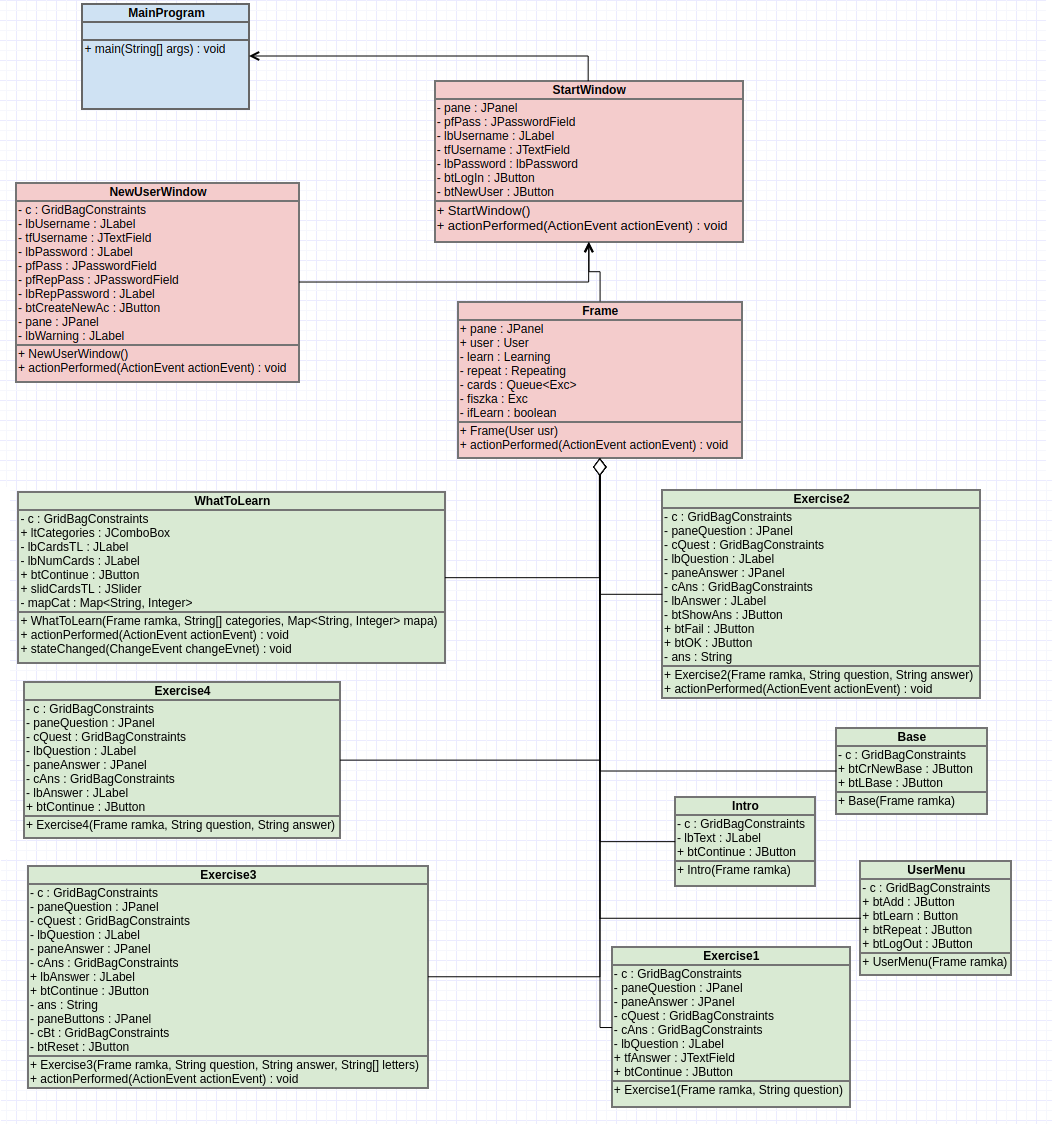
\includegraphics[width=1\linewidth]{diagram.png}

\section{Wzorzec projektowy}

W mojej części projektu LearnIt można zidentyfikować wzorzec \textit{Fasada}. Napisany przez mnie interfejs towrzy właśnie fasadę, za pomocą której użytkownik może komunikować się z bazą danych oraz oraz kolejką przechowującą kolejne fiszki. Nie występuje tutaj dziedziczenie pomiędzy stworzonymi przeze mnie klasami (rozszerzają one tylko gotowe \textit{JFrame} i \textit{JPanel} z biblioteki Swing), natomiast wykorzystują funkcje stworzone przez Julię Majkowską i Agnieszkę Dudek.

\section{Inne zastosowania}

Klasy odpowiadające za logowanie się do systemu można wykrzystać do logowania się na konta w dowolnym projekcie. Wystarczy tylko podać odpowiednią bazę danych oraz okno, które ma zostać wyświetlone po udanym zalogowaniu. \\
Ponadto można zauważyć, że projekt jest przystowsowany do rozszerzeń. W łatwy sposób można dodać nowy rodzaj ćwiczenia oraz dodać go zestawu ćwiczeń w trybie \textit{Learn}.

\end{document}